% Rebuilt by scripts/render.py; edit generator to preserve regeneration.
\documentclass[border=0pt]{standalone}
\usepackage[T1]{fontenc}
\usepackage{mathptmx}
\usepackage{tikz}
\usetikzlibrary{arrows.meta}
\pdfinfoomitdate=1
\pdftrailerid{}
\pdfsuppressptexinfo=15
\definecolor{ink}{HTML}{222222}
\definecolor{accent}{HTML}{4C6E9E}
\definecolor{mid}{HTML}{777777}
\definecolor{rule}{HTML}{D0D3D6}
\newcommand{\dreal}{D_{\mathrm{real}}}
\newcommand{\rtarget}{R_{\mathrm{target}}}
\newcommand{\microv}{V_k^{\mathrm{micro}}}
\newcommand{\vtwo}{V_2^{\mathrm{micro}}}
\begin{document}
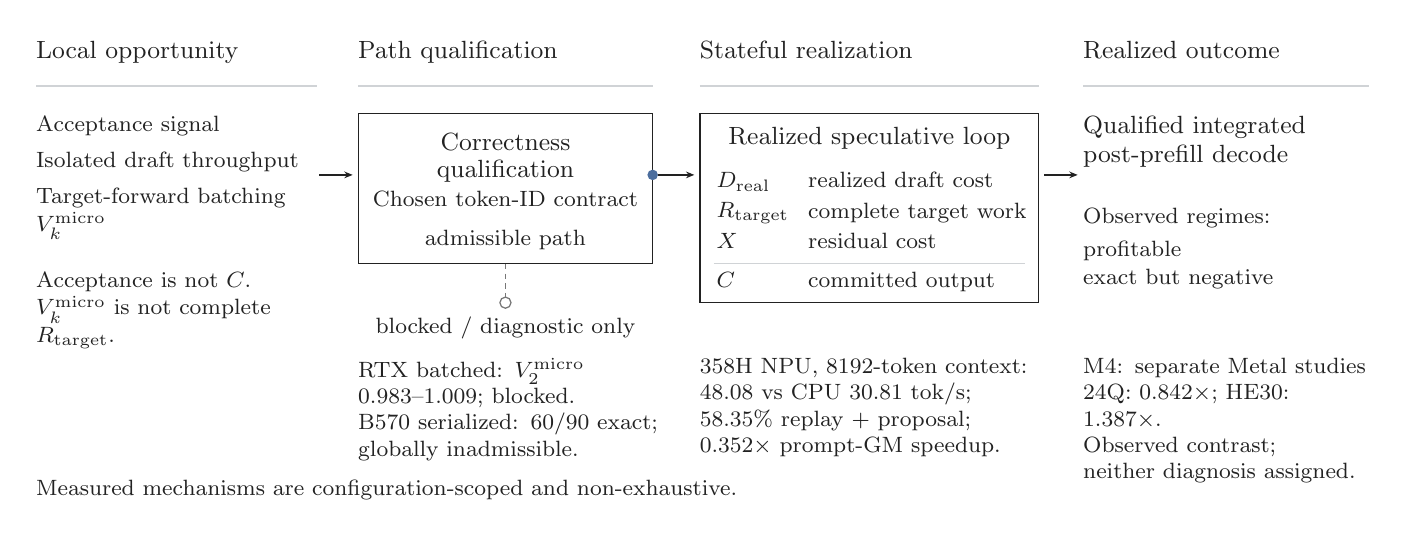
\begin{tikzpicture}[x=1bp,y=-1bp,inner sep=0,outer sep=0,text=ink,line width=.45bp]
\path[use as bounding box] (0,0) rectangle (486,172.8);
\node[anchor=north west,align=left,font=\fontsize{9.2}{11}\selectfont] at (3,5) {Local opportunity};
\draw[rule] (3,21) -- (104,21);
\node[anchor=north west,align=left,font=\fontsize{9.2}{11}\selectfont] at (119,5) {Path qualification};
\draw[rule] (119,21) -- (225,21);
\node[anchor=north west,align=left,font=\fontsize{9.2}{11}\selectfont] at (242,5) {Stateful realization};
\draw[rule] (242,21) -- (364,21);
\node[anchor=north west,align=left,font=\fontsize{9.2}{11}\selectfont] at (380,5) {Realized outcome};
\draw[rule] (380,21) -- (483,21);
\node[anchor=north west,align=left,font=\fontsize{8.5}{10.0}\selectfont,text width=101bp] at (3,32) {Acceptance signal\\[3bp]Isolated draft throughput\\[3bp]Target-forward batching\\$\microv$};
\node[anchor=north west,align=left,font=\fontsize{8}{10}\selectfont,text width=101bp] at (3,88) {Acceptance is not $C$.\\$\microv$ is not complete $\rtarget$.};
\draw[ink] (119,31) rectangle (225,85);
\node[anchor=north,align=center,font=\fontsize{8.8}{10}\selectfont,text width=96bp] at (172,38) {Correctness qualification};
\node[anchor=north,align=center,font=\fontsize{8}{10}\selectfont,text width=99bp] at (172,59) {Chosen token-ID contract};
\node[anchor=north,align=center,font=\fontsize{8}{10}\selectfont,text width=96bp] at (172,73) {admissible path};
\draw[ink,-{Stealth[length=3bp,width=2.4bp]}] (105,53) -- (117,53);
\fill[accent] (225,53) circle[radius=1.9bp];
\draw[ink,-{Stealth[length=3bp,width=2.4bp]}] (227,53) -- (240,53);
\draw[mid,dash pattern=on 2bp off 1.5bp] (172,85) -- (172,99);
\draw[mid,fill=white] (172,99) circle[radius=2bp];
\node[anchor=north,align=center,font=\fontsize{8}{9.5}\selectfont,text width=108bp] at (172,104) {blocked / diagnostic only};
\draw[ink] (242,31) rectangle (364,99);
\node[anchor=north,align=center,font=\fontsize{8.8}{10}\selectfont,text width=116bp] at (303,36) {Realized speculative loop};
\node[anchor=north west,align=left,font=\fontsize{8.5}{10}\selectfont] at (248,52) {$\dreal$};
\node[anchor=north west,align=left,font=\fontsize{8.3}{10}\selectfont] at (281,52) {realized draft cost};
\node[anchor=north west,align=left,font=\fontsize{8.5}{10}\selectfont] at (248,63) {$\rtarget$};
\node[anchor=north west,align=left,font=\fontsize{8.3}{10}\selectfont] at (281,63) {complete target work};
\node[anchor=north west,align=left,font=\fontsize{8.5}{10}\selectfont] at (248,74) {$X$};
\node[anchor=north west,align=left,font=\fontsize{8.3}{10}\selectfont] at (281,74) {residual cost};
\node[anchor=north west,align=left,font=\fontsize{8.5}{10}\selectfont] at (248,88) {$C$};
\node[anchor=north west,align=left,font=\fontsize{8.3}{10}\selectfont] at (281,88) {committed output};
\draw[rule] (247,85) -- (359,85);
\draw[ink,-{Stealth[length=3bp,width=2.4bp]}] (366,53) -- (378,53);
\node[anchor=north west,align=left,font=\fontsize{8.8}{10.5}\selectfont,text width=103bp] at (380,32) {Qualified integrated\\post-prefill decode};
\node[anchor=north west,align=left,font=\fontsize{8.5}{10}\selectfont,text width=103bp] at (380,65) {Observed regimes:\\[2bp]profitable\\exact but negative};
\node[anchor=north west,align=left,font=\fontsize{8}{9.5}\selectfont,text width=108bp] at (119,119) {RTX batched: $\vtwo$\\0.983--1.009; blocked.\\B570 serialized: 60/90 exact;\\globally inadmissible.};
\node[anchor=north west,align=left,font=\fontsize{8}{9.5}\selectfont,text width=130bp] at (242,119) {358H NPU, 8192-token context:\\48.08 vs CPU 30.81 tok/s;\\58.35\% replay + proposal;\\0.352$\times$ prompt-GM speedup.};
\node[anchor=north west,align=left,font=\fontsize{8}{9.5}\selectfont,text width=103bp] at (380,119) {M4: separate Metal studies\\24Q: 0.842$\times$; HE30: 1.387$\times$.\\Observed contrast;\\neither diagnosis assigned.};
\node[anchor=north west,align=left,font=\fontsize{8}{9}\selectfont] at (3,162.8) {Measured mechanisms are configuration-scoped and non-exhaustive.};
\end{tikzpicture}
\end{document}
